\documentclass[a4paper]{article}

\usepackage[spanish]{babel}
\usepackage{graphicx}
\usepackage{amsmath, amssymb}
\usepackage[margin=2cm]{geometry}
\usepackage{fancyhdr}
\usepackage{enumerate}
\usepackage[shortlabels]{enumitem}
\usepackage{parskip}
\usepackage[most]{tcolorbox}
\usepackage[hidelinks]{hyperref}
\usepackage{float}


% cabecera
\pagestyle{fancy}
\fancyhead[l]{Daniel Soto}
\fancyhead[c]{Problemas de Astronomía \#6}
\fancyhead[r]{\today}
\fancyfoot[c]{\thepage}
\renewcommand{\headrulewidth}{0.2pt} % linea horizontal

%% Definicion de comandos para formato de unidades fisicas %%
\newcommand{\m}{\text{m}}
\newcommand{\cm}{\text{cm}}
\newcommand{\km}{\text{km}}
\newcommand{\s}{\text{s}}
\newcommand{\N}{\text{N}}
\newcommand{\g}{\text{g}}
\newcommand{\kg}{\text{kg}}
\newcommand{\Msolar}{\text{M}_\odot}
\newcommand{\Mterrestre}{\text{M}_\oplus}
\newcommand{\AU}{\text{AU}}
\newcommand{\ly}{\text{ly}}
\newcommand{\nT}{\text{nT}}
\newcommand{\GeV}{\text{GeV}}
\newcommand{\atomscm}{\text{atoms/cm}^3}

\newcounter{problema}

\newtcolorbox[use counter=problema]{problema}[1][]{%
    breakable,
    colback=gray!15,
    colframe=gray!60,
    fonttitle=\bfseries,
    title={Problema~\theproblema:},
    boxrule=0.5mm,
    arc=3mm,
    boxsep=5pt,
    left=8pt,
    right=8pt,
    top=6pt,
    bottom=6pt,
    #1
}


\begin{document}

\begin{problema}
 
\textbf{Agujeros negros estelares más cercanos:} ¿Qué tan cerca está el agujero negro más cercano a nuestro Sol? Dado que nuestra galaxia, la Vía Láctea, es un disco muy plano de estrellas, podemos usar coordenadas cartesianas para trazar la ubicación de los agujeros negros más cercanos.

    \begin{figure}[H]
        \centering
        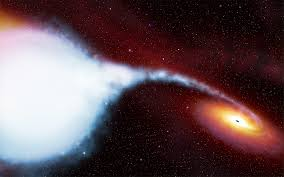
\includegraphics[width=0.7\textwidth]{CygnusX1.jpg}
        \caption{Representación artística del sistema binario Cygnus X-1. A la izquierda, una estrella masiva y brillante pierde materia que es atraída por el agujero negro, formando un disco de acreción incandescente. 
        La materia calentada a millones de grados emite rayos X, lo que convierte a Cygnus X-1 en una de las fuentes más intensas de este tipo de radiación en el cielo.}
        \label{fig:1}
    \end{figure}


Los agujeros negros se crean cuando estrellas muy masivas explotan como supernovas. Afortunadamente, esto no ocurre con mucha frecuencia en nuestra región de la Vía Láctea, ¡por lo que los agujeros negros están realmente muy separados!

La tabla siguiente proporciona las coordenadas de los siete agujeros negros más cercanos a nuestro Sol. La masa de cada agujero negro se da en unidades de masa solar, de modo que 16 significa que la masa del agujero negro es 16 veces la masa de nuestro Sol. Todas las distancias $(x, y, d)$ se dan en años luz, donde 1 año luz = 9.6 billones de kilómetros.

\begin{table}[H]
\centering
\begin{tabular}{|l|c|c|c|c|c|}
\hline
\textbf{Nombre} & \textbf{Masa ($\Msolar$)} & \textbf{x ($\ly$)} & y \textbf{($\ly$)} & \textbf{d (\ly)} \\
\hline
A) Cygnus X-1 & 16 & 6600 & -2400 &  \\
\hline
B) SS-433 & 11 & 8000 & -14000 &  \\
\hline
C) Nova Monocerotis 1975 & 11 & -1400 & 2400 &  \\
\hline
D) Nova Persei 1992 & 5 & 5600 & 3300 &  \\
\hline
E) IL Lupi & 9 & 6500 & -11000 &  \\
\hline
F) Nova Vulpeculi 1988 & 8 & 2200 & -6100 &  \\
\hline
G) V404 Cygni & 12 & 6900 & -4000 &  \\
\hline
\end{tabular}
\caption{Coordenadas de los siete agujeros negros más cercanos al Sol.}
\label{tab:1}
\end{table}

\begin{enumerate}
	\item Cree una cuadrícula de coordenadas cartesianas con el Sol en el origen.
	 En esta cuadrícula, marque la ubicación de cada agujero negro mostrado en la tabla anterior.
	 \item Determine la distancia de cada agujero negro al sol y agreguelo en la tabla.
	 \item ¿Cuál es la distancia media, mediana y modal entre los agujeros negros estelares más cercanos en la vecindad de nuestro Sol?
\end{enumerate}

\end{problema}
[1] \cite{NASA_BlackHoleMath}


\begin{problema}
Los agujeros negros son tan increíblemente densos que enormes cantidades de materia pueden comprimirse en volúmenes muy pequeños. 
Ningún evento físico conocido puede hacer que los agujeros negros sean más pequeños que la masa de una estrella pequeña. 
Pero como los agujeros negros son un producto de la gravedad, al menos teóricamente, no hay límite para lo grande o lo pequeño que pueden ser.

La tabla a continuación muestra el radio predicho de agujeros negros que contienen diversas cantidades de materia. 
Ninguno de estos agujeros negros ha sido observado, pero sus tamaños se han determinado a partir de sus masas declaradas. 
Las masas se dan todas en términos de la masa de nuestra Tierra $\Mterrestre$, $\sim 5.7 \times 10^{24}\kg$, 
de modo que  $2 \Mterrestre$ significa la masa de un agujero negro con el doble de la masa de nuestra Tierra.

\begin{table}[H]
\centering
\begin{tabular}{|c|c|}
\hline
\textbf{Masa ($\Mterrestre$)} & \textbf{Radio ($\cm$)} \\
\hline
2.0 & 16.8  \\
\hline
3.2 & 26.9  \\
\hline
5.0 & 42.0  \\
\hline
7.5 & 63.0  \\
\hline
8.7 & 73.1  \\
\hline
11.0 & 96.6  \\
\hline
\end{tabular}
\caption{Radio predicho de agujeros negros con diferentes masas.}
\label{tab:2}
\end{table}

\begin{enumerate}
	\item Grafique los datos de la tabla.
	\item A partir de la gráfica, use cualquier método para calcular la pendiente, $s$, de los datos. ¿Cuáles son las unidades físicas para el valor de esta pendiente?
	\item A partir de la tabla, calcule la pendiente, S, de los datos.
	\item Escriba una ecuación lineal de la forma $r(m) = s m + r_0$ que exprese la Ley de Masa-Radio del agujero negro.
	\item ¿Qué predeciría como el radio de un agujero negro con la masa del planeta Júpiter, si la masa de Júpiter es 318 veces la masa de la Tierra?
\end{enumerate}

\end{problema}
[3] \cite{NASA_BlackHoleMath}


\bibliographystyle{plainurl}
\bibliography{bibliografia} % Nombre del .bib

\end{document}
